\section{Methodology and Experimental Design}

\subsection{Preliminary Subtopic Clustering Trials}

Before deciding the final the top-down categorical framework, an exploratory bottom-up clustering analysis was performed on the granular subtopics. The objective was to determine if these subtopics would naturally aggregate into distinct, non-overlapping thematic clusters that could independently validate the proposed \gls{spt} dimensions.

%\subsubsection{Observation of Centroid Distributions}

The preliminary clustering was executed by treating each subtopic's intensity as a coordinate in a high-dimensional space. Upon examining the resulting centroids, it was observed that each cluster center was typically dominated by a specific subtopic belonging to one of the main categories. However, despite this individual identification, the overall boundaries between the clusters remained mathematically indistinct, showing high levels of overlap and low silhouette coefficients.

%\subsubsection{Thematic Volatility and Semantic Drift}
The failure to identify natural groupings through unsupervised clustering can be attributed to the high thematic volatility inherent in natural conversation. Unlike structured text, elderly-bot interactions are characterized by rapid transitions; a user may shift from a biographical anecdote (\textit{History}) to a present health concern (\textit{Health}) or a mention of loneliness (\textit{Relationships}) within a very short temporal window. 

This semantic drift implies that subtopics do not exist in isolated silos throughout a session. Instead, they are interwoven in a way that defies traditional partitioning algorithms. Because the conversation evolves rapidly and topics are often functionally unrelated in the short term, the resulting feature space is too sparse and noisy for a purely bottom-up approach to yield meaningful categories. This finding reinforced the necessity of adopting a theoretically grounded framework (the 3 SPT categories) as an anchor to provide the semantic structure that the raw data, by its conversational nature, does not provide spontaneously.





\subsection{Methodological Research Axes}

The semantic characterization of the corpus was restructured into three main research axes setups, regarding  the architecture of the prompt, the granularity of the numerical scale, and the alignment of the mathematical aggregation of subtopics with human evaluators.

Table \ref{tab:research_axes} outlines these as  high-level objectives, focusing on the trade-offs between prompt specificity, scoring complexity, and data fusion techniques.

%\newpage


\begin{table}[htbp]
\centering
\caption{Research Axes and Methodological Goals.}
\label{tab:research_axes}
\begin{tabular}{@{}lp{5cm}p{5cm}@{}}
\toprule
\textbf{Research Axis} & \textbf{Objective} & \textbf{Focus} \\ \midrule
\textbf{Axis I: Architecture} & Analysis of Prompt Scope. & Individualized vs. Unified prompts. \\
\textbf{Axis II: Granularity} & Evaluation of Scoring Resolution. & Binary vs. Rubric (0-5). \\
\textbf{Axis III: Fusion} & Impact of Aggregation Functions. & Mean, Max, and Hadamard operators. \\ \bottomrule
\end{tabular}
\end{table}

To facilitate the mapping between the computational implementation and the statistical analysis, the following nomenclature was defined for the three variants. These variants represent specific combinations of prompting strategies and scoring resolutions.

\begin{table}[!h]%[ht]%[htbp]
\centering
\caption{Technical nomenclature and configuration of the methodological goals.}
\label{tab:experiment_names_updated}
\begin{tabular}{@{}clllp{4cm}@{}}
\toprule
\textbf{Phase} & \textbf{ID} & \textbf{Scoring} & \textbf{Fusion} & \textbf{Prompt Strategy} \\ \midrule

\textbf{I: Architecture} 
& 1 & Rubric (0--5) & - & Categories: Individual vs. Unified prompts comparison. \\ \midrule

\textbf{II: Scoring} 
& 2 & Binary (0--1) & - & Categories: Evaluation under binary scale. \\
& 3 & Trinary (0--2) & - & Categories: Evaluation under trinary scale. \\
& 4 & Rubric (0--5) & - & Categories: Evaluation under rubric scale. \\ \midrule

\textbf{III: Aggregation} 
& 5 & Binary / Trinary / Rubric & Mean & Subcategories: Mean aggregation across all scoring schemes. \\
& 6 & Binary / Trinary / Rubric & Hadamard & Subcategories: Hadamard fusion across all scoring schemes. \\
& 7 & Binary / Trinary / Rubric & Maximum & Subcategories: Max operator across all scoring schemes. \\ 

\bottomrule
\end{tabular}

\vspace{2mm} % Pequeño espacio entre tabla y nota
\begin{minipage}{0.95\textwidth}
    \small \textit{\textbf{Note on Experimental Design:} While scoring granularity was a primary focus of experiment 2, its re-evaluation within these setups serves as a crucial reinforcement layer. This approach ensures the robustness of the metrics when subjected to varying prompt architectures and fusion mechanisms, cross-validating the consistency of the model's performance across phases.}
\end{minipage}
\end{table}

\newpage

\subsubsection*{Mathematical Definitions for Subtopic Fusion}

\begin{table}[htbp]
\centering
\caption{Mathematical Definitions of Variables for Subtopic Fusion}
\label{tab:variable_definitions}
\begin{tabular}{@{}llp{8cm}@{}}
\toprule
\textbf{Variable} & \textbf{Notation} & \textbf{Description} \\ \midrule
\textbf{Intensity} & $s$ & Raw score assigned by the LLM representing the qualitative depth of disclosure of a subtopic. \\
\textbf{Count}     & $n$ & Total number of sub-dimensions or subtopics associated with a specific macro-category/topic. \\
\textbf{Presence}  & $p$ & Binary indicator ($p \in \{0, 1\}$) where 1 indicates the subtopic is present and 0 indicates absence. \\
\textbf{Subtopic Score} & $Score_{sub}$ & The weighted value of a sub-dimension, typically calculated as $s \times p$. \\
\textbf{Category Score} & $Score_{cat}$ & The final aggregated intensity value for a macro-category (Health, Relationships, or History). \\ \bottomrule
\end{tabular}
\end{table}

In Experiment C, the synthesis of sub-dimensional data into a category-level score is governed by three distinct mathematical approaches (entity definitions in Table \ref{tab:variable_definitions}): 

\begin{enumerate}
\item \textbf{Arithmetic Mean ($\mu$):} Provides a balanced representation of the general intensity across all subtopics within a topic. 

\[
\text{Score}_{cat} = \frac{1}{n} \sum_{i=1}^{n} (s_i \cdot p_{cat,i})
\label{eq:hadamard}
\]

\item \textbf{Hadamard Product ($\odot$):} Used to integrate presence/absence detection with intensity rubrics, effectively filtering the score based on explicit evidence.

\[
\text{Score}_{cat} = \frac{1}{n}\sqrt{\sum_{i=1}^{n} (s_i \cdot p_{cat,i})^2} 
\]
% \frac{1}{n}\sqrt{ (S \odot P)^2 \cdot[1 , 1, ...,1]^T} = \text{Intensity} \odot \text{Presence}


\item \textbf{Maximum Operator ($\max$):} Highlights the most prominent sub-dimension, identifying the peak level of self-disclosure within a specific topic.

\[
\text{Score}_{cat} = \max((s_1 \cdot p_{cat,1}),(s_2 \cdot p_{cat,2}), \dots, (s_n \cdot p_{cat,n}))
\]

\end{enumerate}


































\subsection{LLM-Based Feature Extraction}

First, we begin by defining our core categories ($C_1, C_2, C_3$) and the specific subtopics that constitute each thematic domain. This structural mapping, as detailed in Listing \ref{lst:mapping_categories}, serves as the organizational framework for our analysis, ensuring that each granular sub-dimension is correctly aligned with its corresponding higher-level \gls{spt} category.


\begin{lstlisting}[language=Python, caption={Mapping of Subtopics to SPT Categories.}, label={lst:mapping_categories}, frame=single, basicstyle=\small\ttfamily]
category_mapping = {
    'Category 1: Health and Well-being': [
        'mental_emotional_health', 
        'physical_health_addictions'
    ],
    'Category 2: Interpersonal Relationships': [
        'family_dynamics', 
        'affective_relationships'
    ],
    'Category 3: Personal History and Development': [
        'personal_goals_failures', 
        'traumas_adversities', 
        'professional_career'
    ]}
\end{lstlisting}

With these mathematical foundations established, the previously defined vectors can now be populated with their respective numerical values:

\begin{equation}
\mathbf{S} = [s_1, s_2, s_3, s_4, s_5, s_6, s_7]
\end{equation}

\begin{equation}
\quad \mathbf{P}_1 = \begin{bmatrix} 1 \ 1 \ 0 \ 0 \ 0 \ 0 \ 0 \end{bmatrix}, \quad \mathbf{P}_2 = \begin{bmatrix} 0 \ 0 \ 1 \ 1 \ 0 \ 0 \ 0 \end{bmatrix}, \quad \mathbf{P}_3 = \begin{bmatrix} 0 \ 0 \ 0 \ 0 \ 1 \ 1 \ 1 \end{bmatrix}
\end{equation}


The organization of the feature extraction experiments is summarized in Table \ref{tab:llm_experiments}, which outlines the specific objectives and methodological protocols for each experimental setup.


\begin{table}[htbp]
\centering
\caption{Summary of LLM-Based Feature Extraction Experiments.}
\label{tab:llm_experiments}
\begin{tabular}{@{}lp{6cm}p{4.5cm}@{}}
\toprule
\textbf{Experiment} & \textbf{Objective} & \textbf{Methodology} \\ \midrule

\textbf{4.2.1: Exp. A} & Fine-grained analysis of Subtopics. & Rubric vs. Binary evaluation for individual subtopics. \\

\textbf{4.2.2: Exp. B} & Integration of intensity and presence via Hadamard Product. & Rubric (0-5) $\odot$ Binary (0/1) at subcategory level. \\

\textbf{4.2.3: Exp. C} & Direct comparison of scoring granularity at the Category level. & Rubric vs. Binary evaluation for C1, C2, and C3. \\
 \bottomrule
\end{tabular}
\end{table}



To ensure consistency between the computational implementation and the analytical results, a standardized nomenclature was established for the six experimental variants, as detailed in Table \ref{tab:experiment_names}. These are grouped into three main categories based on their granularity (Category vs. Subtopic) and their scoring logic (Rubric, Binary, or Hadamard Fusion).

\begin{table}[htbp]
\centering
\caption{Technical nomenclature of the experiments conducted.}
\label{tab:experiment_names}
\begin{tabular}{@{}cllp{5cm}@{}}
\toprule
\textbf{Exp.} & \textbf{ID} & \textbf{Technical Name} & \textbf{Description} \\ \midrule
\textbf{A} & 1 & \texttt{rubric based hadamard fusion} & Category-level rubric scores. \\
           & 2 & \texttt{binary hadamard fusion} & Category-level scores from binary flags. \\ \midrule
\textbf{B} & 3 & \texttt{topic rubric} & Direct evaluation of the 3 main categories using a 0-5 scale. \\
           & 4 & \texttt{topic binary} & Direct presence/absence detection of the 3 main categories. \\ \midrule
\textbf{C} & 5 & \texttt{subtopic rubric} & Detailed 0-5 scoring for each specific subtopic. \\
           & 6 & \texttt{subtopic binary} & Presence/absence detection for each specific subtopic. \\ \bottomrule
\end{tabular}
\end{table}

\newpage

\textbf{Experiment B} represents our primary approach, where we hypothesize that multiplying the rubric score by binary flag vectors (defined as Presence $P$) to later apply the Hadamard Product, that filters out low-confidence model assignments while preserving the intensity of high-quality disclosures.\\
\textbf{Experiments A and C} serve as ablation studies and validation baselines to justify the complexity of the feature engineering process.



        \subsubsection{Experiment A: Subtopics (Rubric vs Binary)}
The experimental workflow follows a bottom-up structure, beginning with Experiment C (Sub\-to\-pics) due to a critical data dependency. This experiment serves as the foundational feature extraction layer; it is a mathematical prerequisite to obtain granular scores for each specific sub-dimension before executing higher-level operations.

The evaluation of subtopics was performed with a zero-shot/few-shot hybrid prompt. This prompt defines the semantic boundaries for each of the seven subtopics and establishes a rigorous scoring rubric. This prompt is described in Annex \ref{appendix:prompt_subtopics}.

For the binary variant of Experiment C, the model's instructions were simplified to a detection task. The prompt explicitly forbids intermediate values, forcing a strictly boolean output (0 or 1). This reduction in dimensionality serves to minimize variance and provide a high-confidence indicator of thematic occurrence (See Appendix \ref{appendix:prompt_subtopics}).

        
        \subsubsection{Experiment B: Rubric-Based vs. Binary Scoring via Hadamard Product}

The hadamard product is used to merge the qualitative depth of the scores.

First, the gating mechanism in matrix-vector form is denoted as:

\begin{equation}
    \begin{bmatrix} s_1 \\ s_2 \\ \vdots \\ s_n \end{bmatrix} \odot \begin{bmatrix} p_1 \\ p_2 \\ \vdots \\ p_n \end{bmatrix} = \begin{bmatrix} s_1 \cdot p_1 \\ s_2 \cdot p_2 \\ \vdots \\ s_n \cdot p_n \end{bmatrix}
\end{equation}

By substituting the components of the Hadamard product ($f_i = s_i \cdot p_i$), the final operational formula for Experiment B becomes:\begin{equation}S_{cat} = \frac{1}{n}\sqrt{\sum_{i=1}^{n} (s_i \cdot p_i)^2}\end{equation}

% This approach implements a \textit{gating mechanism} where the binary vector $\mathbf{P}$ validates the presence of the category. 



        \subsubsection{Experiment C: Direct Category Evaluation (Rubric vs Binary)}

The rubric-based prompt  for Experiment C (See Appendix \ref{appendix:prompt_categories}) provides the model with a nuanced scale to differentiate between impersonal mentions and deep emotional vulnerability. This allows for a direct comparison with the aggregated results of Experiment A to determine if "direct inference" leads to a loss of granularity. 
        
The prompt for Experiment C (Binary) (also in Appendix \ref{appendix:prompt_categories}) instructs the model to act as a high-level classifier. Unlike the subtopic prompt, this prompt requires the LLM to perform an internal aggregation, considering various aspects (e.g., physical health and emotional state) under a single categorical label.


%\subsection{Programmatic Feature Extraction}

%In addition to the semantic analysis, a programmatic extraction phase was conducted to capture the structural and emotional nuances of the interactions. These features provide a quantitative baseline for characterizing user behavior.

%\begin{itemize}
%    \item \textbf{Interaction Metrics:} Columns such as \texttt{n\_user\_interactions},\\ \texttt{percentage\_user\_interactions}, and \texttt{len\_user\_interactions} were calculated using custom scripts to measure the user's conversational engagement and verbosity.
    
%    \item \textbf{Sentiment Analysis:} We utilized the \textit{Pysentimiento} library to extract the emotional polarity (\texttt{pos}, \texttt{neu}, \texttt{neg}) of both the user and the bot. This allows for the identification of emotional trends and the assessment of the bot's empathetic alignment.
    
%    \item \textbf{Named Entity Recognition (NER):} Using the \textit{SpaCy} framework, we quantified the frequency of proper nouns (\texttt{n\_proper\_nouns}) in the user's speech. A higher density of entities (e.g., family names or specific locations) serves as a proxy for the specificity and depth of the narrative.
%\end{itemize}


%\subsection{Clustering Strategy}


\subsection{Unsupervised Machine Learning}
\label{sec:metrics_label}
Unsupervised machine learning comprises a set of techniques designed to identify underlying structures and patterns in datasets that lack explicit labels. In the context of this thesis, where the objective is to categorize the depth of 16,000 spontaneous interactions without a pre-existing %\textit{Gold Standard}, 
annotation, this paradigm provides a scalable and objective framework for behavioral discovery.

Following the comprehensive review in \cite{Naeem2023}, unsupervised learning is fundamental for exploratory data analysis, as it allows for the identification of natural groupings based on feature proximity in a multi-dimensional space. The utility of this approach in social computing lies in its ability to handle high-dimensional semantic vectors—such as those extracted via LLMs—and organize them into interpretable clusters without human bias influencing the initial grouping process.



A critical component of unsupervised learning is the evaluation of the resulting data partitions. Since there is no external label to compare against, in \cite{Naeem2023} internal validation criteria are emphasized to measure clustering quality:
\begin{itemize}
    \item \textbf{Cohesion:} Measures the degree to which elements within a cluster are similar to one another.
    \item \textbf{Separation:} Evaluates the distinctness between different clusters to ensure they represent unique categories.
    \item \textbf{Validation Metrics:} Indicators such as the \textit{Silhouette Score} (measuring point-to-cluster assignment quality) and the \textit{Davies-Bouldin Index} (evaluating the ratio of within-cluster to between-cluster distances)  assess the mathematical validity of the model.
\end{itemize}

This theoretical grounding makes clustering a suitable tool for mapping conversational data to the layers of SPT, providing the necessary metrics to evaluate whether the extracted features are capable of forming stable and meaningful representations of user behavior.
    
        
\subsubsection{K-Means Clustering %and Evaluation Metrics employed
}

K-Means is an unsupervised learning technique to partition $n$ observations into $K$ clusters, where each observation belongs to the group with the nearest mean (centroid). The mathematical objective is to minimize the \textit{Within-Cluster Sum of Squares} (WCSS):

\begin{equation}
    J = \sum_{j=1}^{K} \sum_{x_i \in C_j} \|x_i - \mu_j\|^2
\end{equation}

To evaluate the validity of the partition and select the optimal number of clusters, this study employs the following metrics and heuristics based on \cite{Naeem2023}:

\begin{itemize} 
    \item \textbf{Elbow Method:} Identification of the inflection point in the WCSS curve.
    \item \textbf{Silhouette Score:} A measure of cohesion and separation ranging from -1 to 1.
%    \item \textbf{Calinski-Harabasz Index:} The ratio of the sum of between-clusters scatter and within-cluster scatter.
%    \item \textbf{Davies-Bouldin Index:} The average maximum similarity index of each cluster with another; lower values signify better separation.
%    \item \textbf{Gap Statistics:} A statistical technique that compares cluster dispersion with a uniform reference distribution.
\end{itemize}

% --- Tabla de Métricas para el Estado del Arte ---
\begin{table}[htbp]
\centering
\caption{Summary of Clustering Evaluation Metrics and Optimal Selection Criteria.}
\label{tab:clustering_metrics_simple}
\begin{tabular}{@{}ll@{}}
\toprule
\textbf{Metric / Method} & \textbf{Optimal Value Criterion} \\ \midrule
Elbow Method             & "Knee" or Inflection point       \\
Silhouette Score         & Maximize ($\to 1$)               \\
%Calinski-Harabasz Index  & Maximize                         \\
%Davies-Bouldin Index     & Minimize                         \\
%Gap Statistics           & Maximize                         \\
%GMM - BIC                & Minimize                         \\
%DBSCAN                   & Density-based (Variable)         \\ 
\bottomrule
\end{tabular}
\end{table}
% ------------------------------------------------

%Furthermore, this study considers \textbf{Gaussian Mixture Models (GMM)} evaluated through the \textbf{Bayesian Information Criterion (BIC)} to balance likelihood and parsimony. Finally, we contrast these with \textbf{DBSCAN}, a density-based approach. While DBSCAN is effective at identifying outliers, it may struggle with the varying densities of semantic layers, reinforcing the choice of a centroid-based approach for the thematic categorization required by Social Penetration Theory.



\subsubsection{Dimensionality Reduction and Visualization}

%The feature vectors extracted from the \textit{Gemma-2-9b-it} model reside in a high-dimensional latent space, which can hinder the performance of centroid-based clustering. To address this, two complementary techniques are integrated into the analytical pipeline: Principal Component Analysis (PCA) and t-Distributed Stochastic Neighbor Embedding (t-SNE).

%\textbf{Principal Component Analysis (PCA)} is applied as a deterministic dimensionality reduction step. By performing an eigendecomposition of the covariance matrix, PCA projects the semantic features into a lower-dimensional space that retains the highest possible variance. This reduction not only decreases the computational burden on the K-Means algorithm but also filters out redundant information, emphasizing the primary dimensions of user self-disclosure.

%hile PCA preserves global variance, \textbf{t-SNE} is employed for its superior ability to represent local relationships in a visualizable 2D space. t-SNE converts similarities between data points into joint probabilities and seeks to minimize the Kullback-Leibler divergence between the original and the low-dimensional distributions. In this research, t-SNE serves as a qualitative validation tool, allowing for the visual inspection of the clusters and ensuring that the mathematical partitions reflect coherent patterns of interaction between the elderly users and the chatbot.


The feature vectors extracted are processed within their original high-dimensional latent space to ensure the theoretical integrity of the SPT categories. To avoid the loss of granular information, K-Means clustering is applied directly to the extracted features without prior reduction. Consequently, dimensionality reduction techniques are used strictly for \textit{post-hoc} analysis and visualization.

Principal Component Analysis (PCA) is implemented as a deterministic validation tool. By projecting the dataset into its primary eigenvectors, PCA allows for the inspection of the global data structure and the verification of cluster separability based on maximum variance.

Furthermore, t-Distributed Stochastic Neighbor Embedding (t-SNE) is utilized to represent complex, non-linear local relationships in a 2D plane. %In this pipeline, t-SNE serves exclusively as a qualitative visual aid. It is crucial to denote 
We remark that neither PCA nor t-SNE are used to feed the clustering algorithm; their role is to provide a human-interpretable validation of the high-dimensional mathematical partitions, ensuring they reflect coherent interaction patterns.



\begin{table}[htbp]
\centering
\caption{Comparison between PCA and t-SNE for Dimensionality Reduction.}
\label{tab:pca_vs_tsne}
\begin{tabular}{@{}lll@{}}
\toprule
\textbf{Feature}          & \textbf{PCA}                  & \textbf{t-SNE}                 \\ \midrule
\textbf{Type}             & Linear                        & Non-linear                     \\
\textbf{Data Preservation}& Global structure (Variance)   & Local structure (Similarity)   \\
\textbf{Computational Cost}& Low / Efficient               & High / Iterative               \\
\textbf{Determinism}      & Deterministic                 & Stochastic (Non-deterministic) \\
\textbf{Output}           & Principal Components          & Low-dimensional clusters       \\
\textbf{Main Use Case}    & Noise reduction / Processing  & Data visualization             \\ \bottomrule
\end{tabular}
\end{table}












       \subsubsection{Implementation of the K-Means Algorithm}
The clustering phase was executed using the K-Means algorithm, chosen for its interpretability in centroid analysis. The model was applied directly to the feature space to maintain the SPT. While the Silhouette Coefficient and Elbow Method results were not entirely decisive (suggesting a continuous distribution of user behaviors), the algorithm successfully identified core trends in the data.

\begin{figure}[htbp]
    \centering
    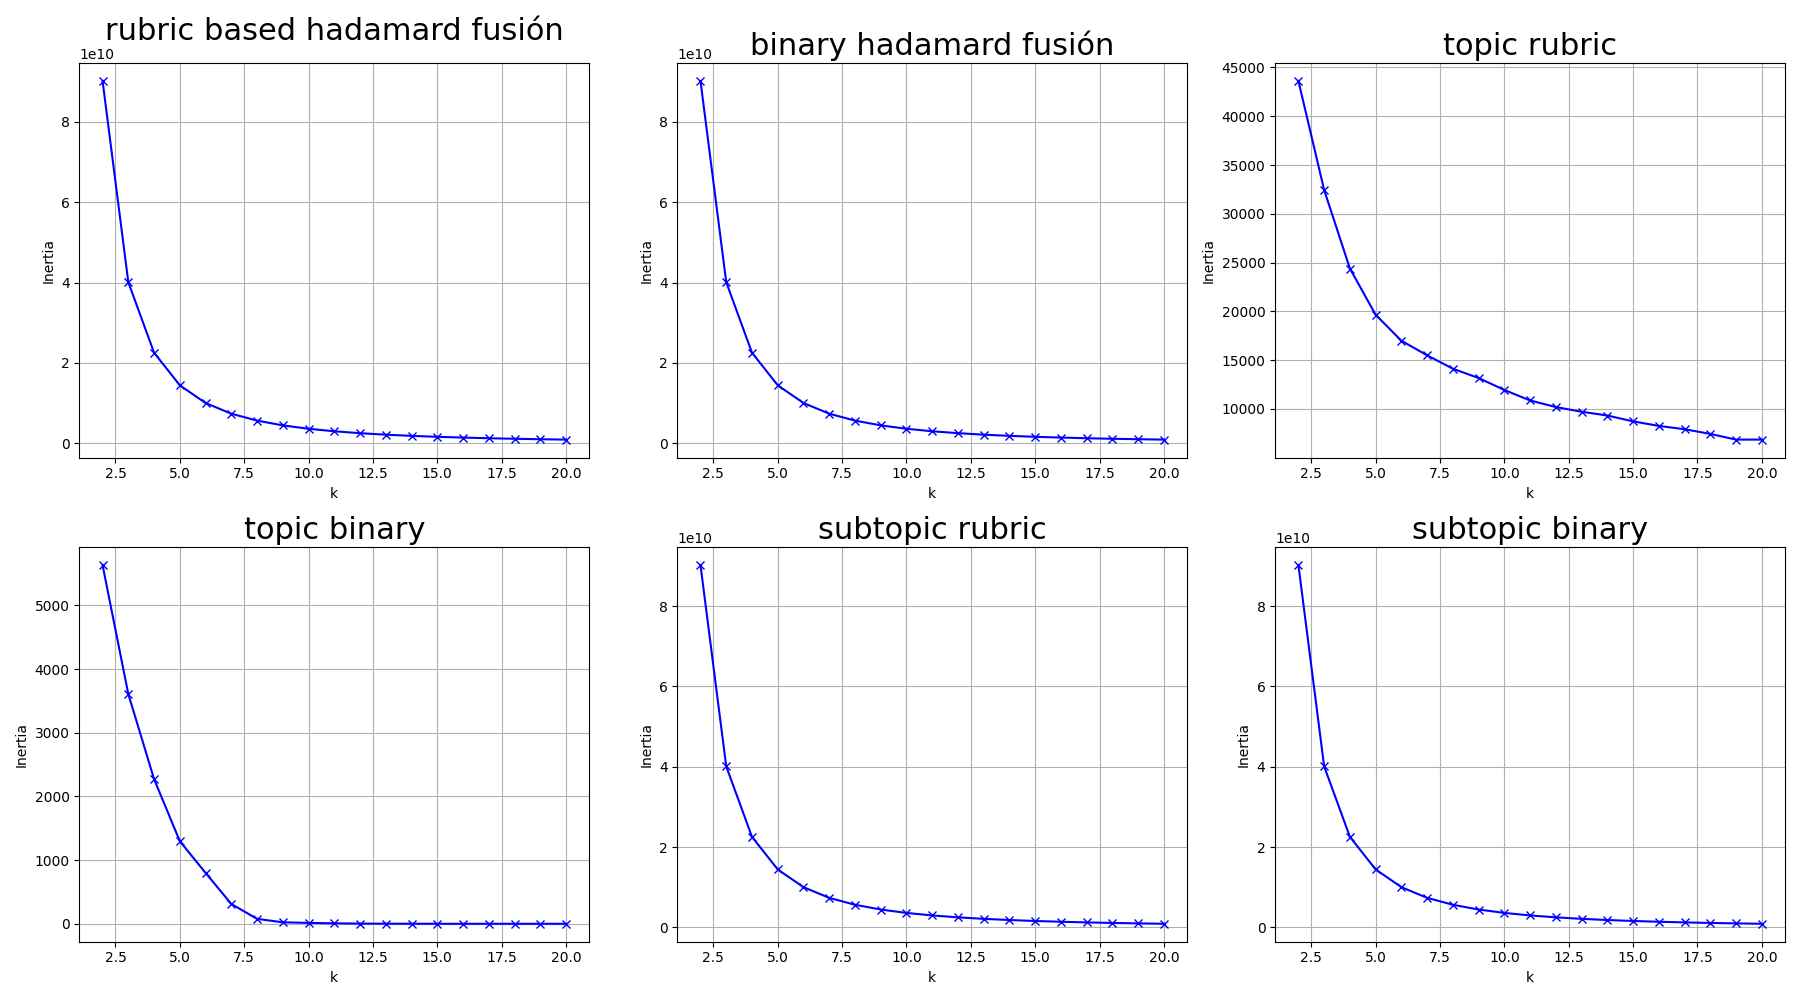
\includegraphics[width=0.9\textwidth]{images/6codos.png}
    \caption{Elbow Method analysis for cluster optimization. }
    \label{fig:elbow_method}
\end{figure}
\newpage

\begin{figure}[htbp]
    \centering
    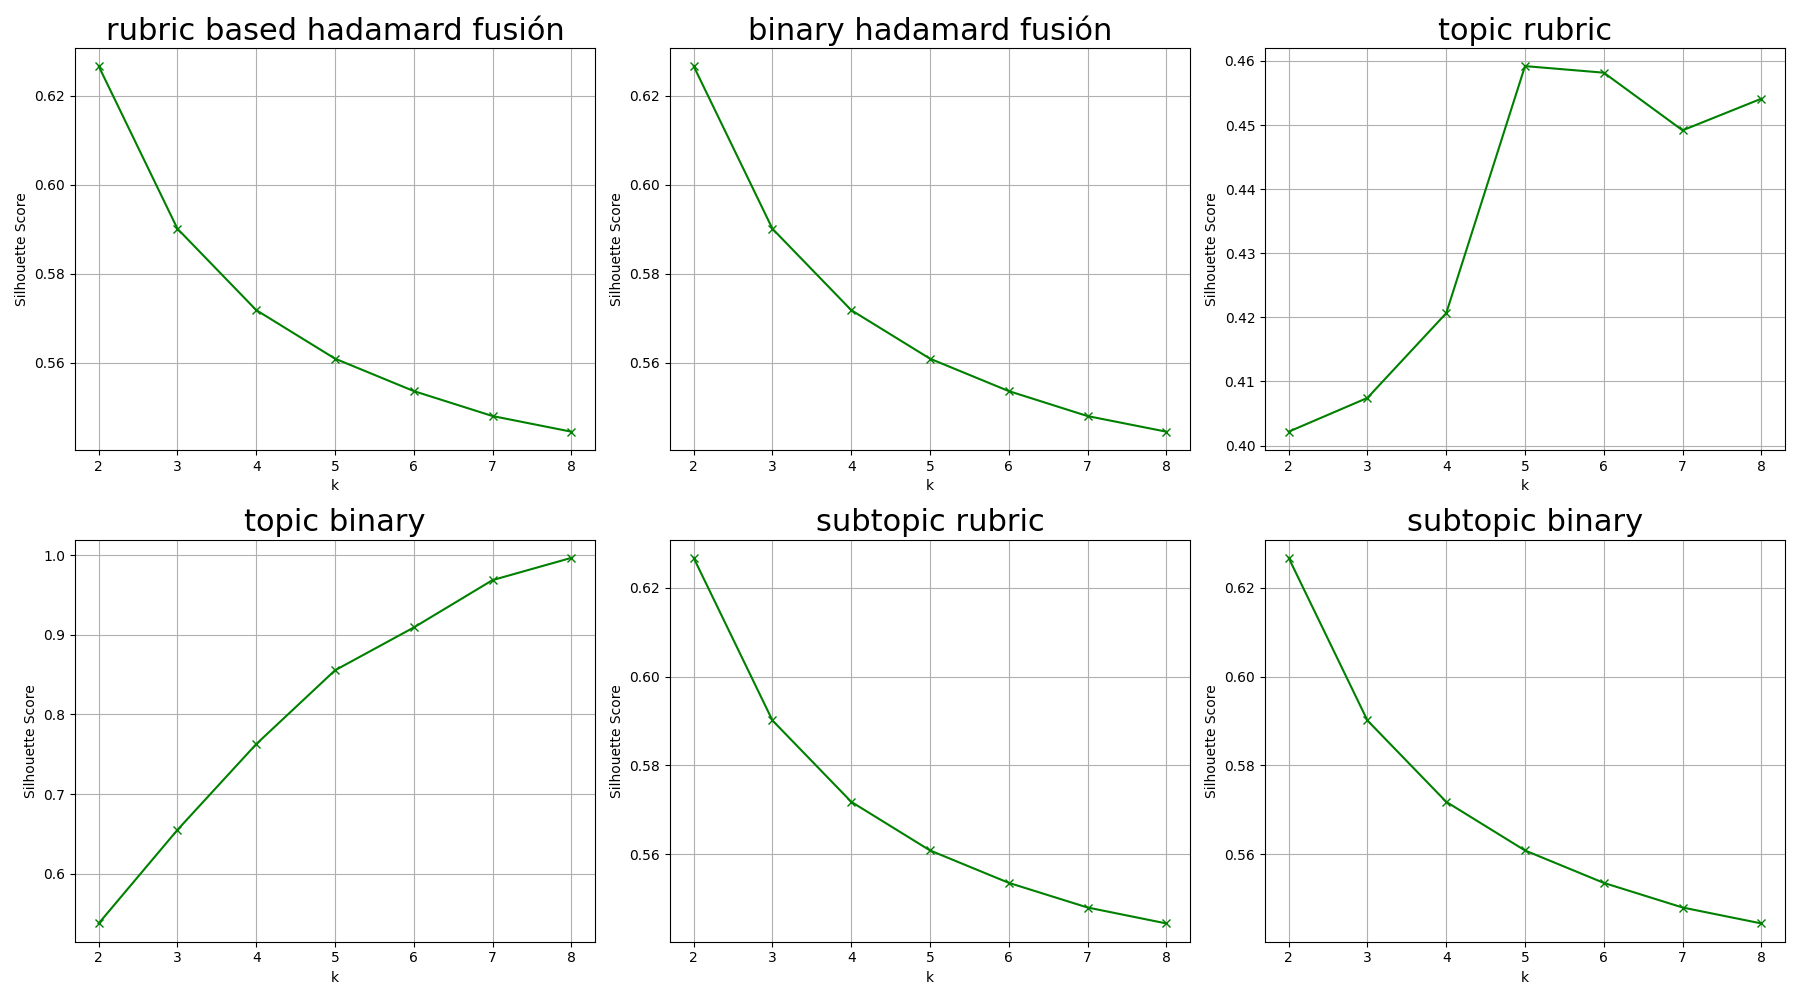
\includegraphics[width=0.9\textwidth]{images/6siluetas.png}
    \caption{Silhouette Method analysis for cluster optimization. }
    \label{fig:silhouette_method}
\end{figure}
As illustrated in Figure \ref{fig:elbow_method}, the inertia curve does not exhibit a clearly defined "elbow" or a sharp inflection point. This lack of a decisive break suggests that the self-disclosure patterns in our elderly-chatbot dataset do not form naturally isolated groups with high density. Instead, the results point towards a behavioral continuum, where the boundaries between different levels of intimacy are fluid and overlapping.
\\
Despite the absence of a mathematically unique optimal $k$, the selection of an \textit{N+1} approach prioritizes  qualitative interpretability over purely mathematical partition metrics. 
%\subsubsection{Justification of a 4-Cluster Approach}
Specifically, we propose a 3+1 cluster approach. The 3 clusters represent the stable behavioral archetypes identified through inference (and they would target the aforementioned $C_1$, $C_2$  and $C_3$). The additional cluster is strategically designed to capture  mixed interactions. This separation is crucial in elderly-bot datasets to prevent ``cold-start" sessions from diluting the semantic clarity of the primary topic centroids. 

































